\section*{Problem 1}
	\begin{enumerate} [1)]
		\item \begin{proof} [Solution]
			The below figure shows the convergence of the sample mean. Decreasing with the rate of $\frac{1}{\sqrt{N}}$.
			\begin{center}
				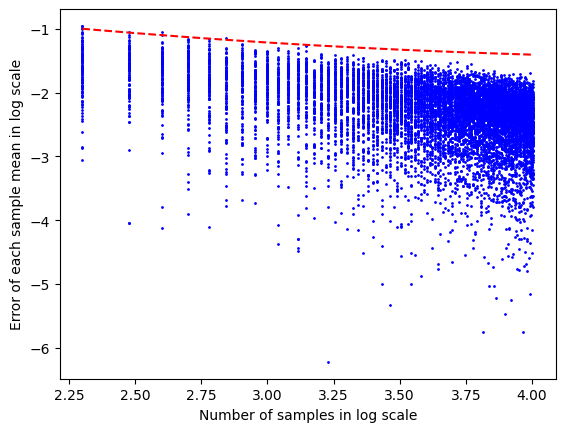
\includegraphics[width=0.4\textwidth]{example.png}
			\end{center}
		\end{proof}
		\item \begin{proof} [Solution]
			Following histograms show the distribution of $\mu_M(N)$ with increasing $M$. We can check it becomes similar to a normal distribution as $M$ goes to $\infty$. Since the exact distribution is a uniform distribution from -1 to 1, $\mu_{\mbox{exact}} = 0$ and $\sigma_{\mbox{exact}} = \sqrt{\frac{1}{3}} \simeq 0.577$. Here is the error.
			\begin{figure} [htb!]
				\centering
				\subfloat[sample histogram]{{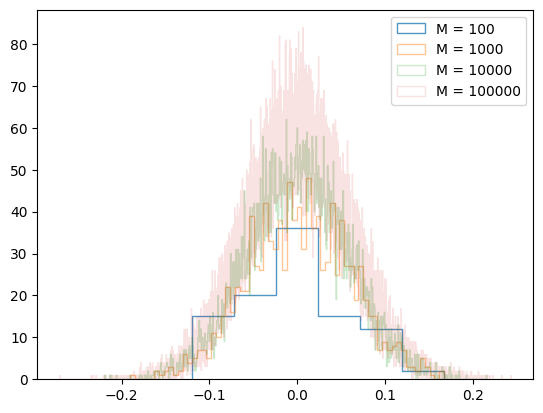
\includegraphics[width=0.4\textwidth]{histo.png}}}
				\subfloat[sample value and error]{{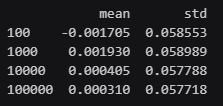
\includegraphics[width=0.4\textwidth]{table.png}}}
			\end{figure}\\
			From this, we can check that $\mu_M \simeq \mu_{\mbox{exact}}$ and $\sigma_M \times 10 \simeq \sigma_{\mbox{exact}}$. Note that the coefficient `10' comes from the sample size $N = 100$.\\
		\end{proof}
		\item \begin{proof} [Solution]
			From 2), we can check that $\sigma_{\mbox{exact}}$ is related to $N$. i.e. $\sigma_M \propto \frac{1}{\sqrt{N}}$. Because of this, the error in 1) converges with rate $\frac{1}{\sqrt{N}}$. This is why the errors of the most trials decay with the rate of $\frac{1}{\sqrt{N}}$.\\
		\end{proof}
	\end{enumerate}